\chapter{Le \textit{\uppercase{L}arge \uppercase{H}adron \uppercase{C}ollider} et le détecteur CMS}
\label{chap4}

La seconde guerre mondiale eut pour conséquence sur l'Europe une fuite des cerveaux vers les États-Unis entraînant la perte de son rayonnement international en matière de recherche en physique. Sur ce constat, plusieurs physiciens notables de l'époque parmi lesquels figurent Edoardo Amaldi, Pierre Auger et Niels Bohr émettent l'idée de la création d'un nouveau laboratoire de recherche en physique nucléaire a l'échelle européenne. Louis de Broglie fut le premier à proposer un tel projet lors de la conférence européenne de la culture à Lausanne en décembre 1949, dont le principal argument retenu sera celui du partage des coûts entre les nations, sans encore bénéficier du soutien des gouvernements. Cette proposition sera suivie d'une seconde en juin 1950 lors de la conférence générale de l'UNESCO à Florence, sous l'impulsion du physicien américain Isidor Rabi, prônant la nécessité d'une collaboration scientifique internationale. En 1951, un conseil provisoire baptisé Conseil Européen pour la Recherche Nucléaire est fondé menant à la ratification en 1954 de la première convention officielle du CERN par 12 nations européennes. Le choix de l'emplacement est porté vers la Suisse pour sa position centrale au sein de l'Europe et sa neutralité, avec la pose de la première pierre à l'édifice sur le site de Meyrin en juin 1955 par Felix Bloch alors directeur général du CERN. \\

Dès 1957 le CERN lance la construction de son premier accélérateur de particules. Il s'agira d'un synchrocyclotron (SC) permettant de conduire un faisceau de protons d'une énergie de $600$ MeV sur une cible fixe, menant à l'observation de la désintégration rare du pion en électron seulement quelques heures après son démarrage en 1958. En 1959, le CERN met en fonction son premier synchrotron à protons (PS, \textit{proton synchrotron}) atteignant une énergie de $28$ GeV et devenant pendant une brève période l'accélérateur le plus puissant du monde devançant de $10$ GeV le record  établi par l'URSS. \\

En 1968, l'invention de la chambre à fils par le physicien français Georges Charpak révolutionne le concept de détection en physique des particules. Le détecteur se compose d'une enceinte remplie de gaz inerte dans laquelle des grilles constituées de fils parallèles sous tension sont empilées par alternance de cathodes et d'anodes. Le passage d'une particule chargée entraîne ainsi l'ionisation du gaz et un déplacement de charges mesurable sous la forme d'une impulsion électrique. Cette technique rend désormais possible le traitement informatique des données et viendra rapidement remplacer les chambres à bulles pour lesquelles une analyse image par image "à la main" des traces produites était nécessaire. \\

Le début des années 70 marque le début des premières collisions proton-proton au sein de l'ISR (\textit{Intersecting Storage Ring}), un nouvel accélérateur alimenté par le PS. Avec une énergie dans le centre de masse de $62$ GeV, le concept de croisement de faisceaux permet un accès à des hautes énergie en produisant le même effet qu'une collision sur cible fixe à une énergie de $2000$ GeV. Durant 13 années d'opération, l'ISR aura notamment permis un sondage profond de la matière en offrant aux physiciens les premiers indices de la nature composite du proton. Il servira également d'instrument pour le développement du refroidissement stochastique inventé par Simon van der Meer, permettant d'augmenter et d'uniformiser significativement la densité d'énergie des faisceaux de particules chargées. En parallèle, le CERN lance son projet de construction du \textit{super proton synchrotron} (SPS), un collisionneur proton-proton sous-terrain d'une circonférence de $7$ km, lancé en 1976. Il sera par la suite converti en collisionneur proton-antiproton en 1979 suivant l'initiative de Carlo Rubia et Simon van der Meer menant à la découverte des bosons $W$ et $Z$ en 1983 par les expériences UA$1$ et UA$2$. \\

L'année 1988 est marquée par l'injection du premier faisceau dans le \textit{Large Electron-Positron} (LEP) \textit{collider}. Ce collisionneur d'une circonférence de $27$ km fut capable de produire des collisions électron-positron à une énergie dans le centre de masse de $100$ GeV à son lancement et jusqu'à $209$ GeV à la fin de son exploitation le 2 novembre 2000. Le LEP servit à réaliser plusieurs mesures de précision notamment de la masse des bosons électrofaibles $W$ et $Z$ \cite{Wmass,Zmass}, et en fixant les premières limites inférieures sur la masse du boson de Higgs avant sa découverte. Il permit également de contraindre à trois le nombre de générations de fermions via la mesure de la largeur de désintégration du boson $Z$ \cite{ZALEPH,ZDELPHI,ZL3,ZOPAL}. Les travaux d'excavation réalisés pour la mise en place de l'accélérateur et de ses expériences servirent ensuite de base à la mise en place de l'actuel \textit{Large Hadron Collider} (LHC) et de ses quatre expériences majeures : CMS, ATLAS, ALICE et LHCb. \\

\section{LHC, \textit{\uppercase{L}arge \uppercase{H}adron \uppercase{C}ollider}}

Le 18 septembre 2008, le premier faisceau de protons est injecté avec succès au sein du LHC d'une circonférence de $27$ km et situé à une profondeur moyenne de $100$ m. Les physiciens se tiennent alors prêts à entrer dans une nouvelle ère de découvertes à des échelles d'énergie jamais atteintes. La machine promet un programme de physique large, allant de la recherche du boson de Higgs et de nouvelles particules s'inscrivant dans une physique \textit{au-delà du modèle standard}, à l'étude de l'évolution de la matière dans les premiers instants de l'Univers.

\subsection{Caractéristiques techniques}

L'injection des deux faisceaux dans le LHC circulant en sens opposés est assurée par un complexe d'accélérateurs constitué de ses prédécesseurs (Fig. \ref{complex}). Au départ, les protons sont issus de dihydrogène duquel les électrons sont arrachés par un champ électrique produit dans un cylindre métallique appelé duoplasmatron. Ils sont ensuite regroupés en paquets et accélérés à une énergie de $750$ keV avant d'être injectés dans un accélérateur linéaire, le LINAC$2$, pour atteindre une énergie de $50$ MeV. Depuis 2020, le LINAC$4$ succède au LINAC$2$ en fournissant un faisceau d'ions $H^-$ porté à une énergie de $160$ MeV. Les protons sont obtenus en arrachant les deux électrons des ions $H^-$ et sont ensuite amenés respectivement à une énergie de $1,4$ GeV en sortie du booster, $26$ GeV en sortie du PS et atteignent finalement $450$ GeV en sortie du SPS au moment de l'injection dans le LHC et avant d'être à nouveau accélérés par $16$ cavités radiofréquence jusqu'à leur énergie nominale. Jusqu'à la fin de la seconde phase d'exploitation du LHC en 2018 (Run 2), chaque faisceau pouvait emporter jusqu'à 2556 paquets de protons eux-mêmes constitués d'une centaine de milliards de protons. Ces chiffres ont été revus à la hausse pour la troisième phase d'exploitation (Run 3) démarrée en 2022 et encore en cours à ce jour en 2023, permettant d'augmenter la quantité de collisions produites aussi appelée \textit{luminosité instantanée}. Celle-ci est définie par : 

\begin{figure}
\centering
    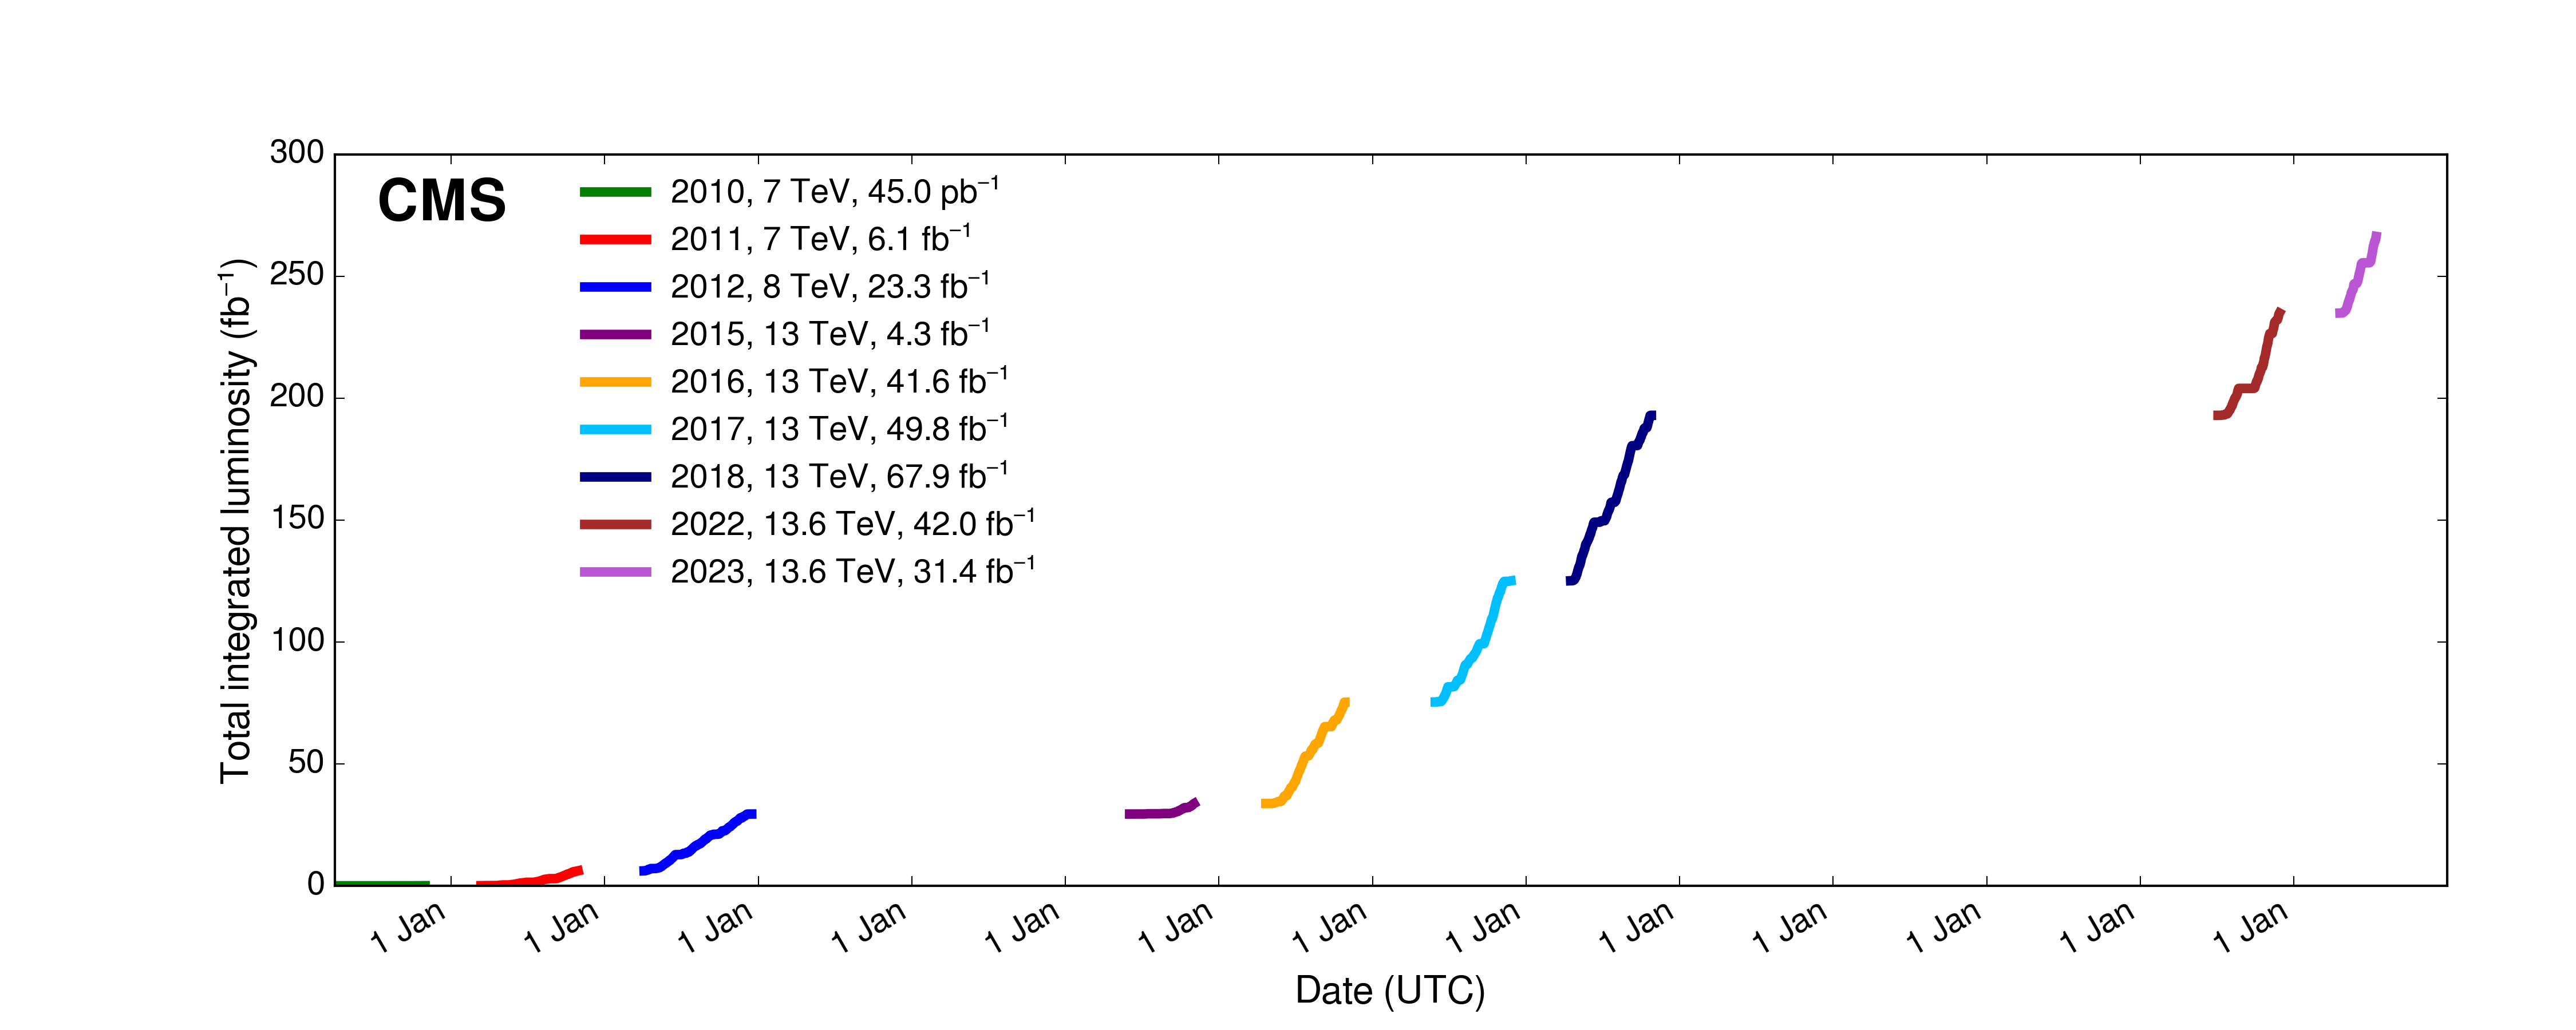
\includegraphics[scale=0.4]{Chapitre3/Images/int_lumi_cumulative_pp_3.png} 
\caption{Luminosité intégrée au cours du temps enregistrée par CMS depuis le lancement du LHC à juillet 2023 \cite{LumiTwiki}.}
\label{lumi}
\end{figure}


\begin{equation}
    \mathcal{L}=\frac{N_pn_bf}{4\pi\sigma_x\sigma_y}F,
\end{equation}

où $N_p$ désigne le nombre de particules par paquets, $n_b$ le nombre de paquets par faisceau, $f$ la fréquence de croisement des faisceaux, $\sigma_{x,y}$ la taille transverse du faisceau selon la coordonnée $x$ ou $y$ et $F$ un correctif lié à l'angle de croisement des faisceaux au point d'interaction. La luminosité instantanée intervient naturellement dans le nombre d'évènements produits au cours du temps selon la formule : 

\begin{equation}
    \frac{\partial N}{\partial t}=\mathcal{L}\times\sigma,
\end{equation}

où $\sigma$ est la section efficace du processus considéré. L'intégration de la luminosité instantanée sur un temps $t$ permet également de connaître la quantité de données enregistrée sur cette période (Fig. \ref{lumi}).  \\

\begin{figure}
\centering
    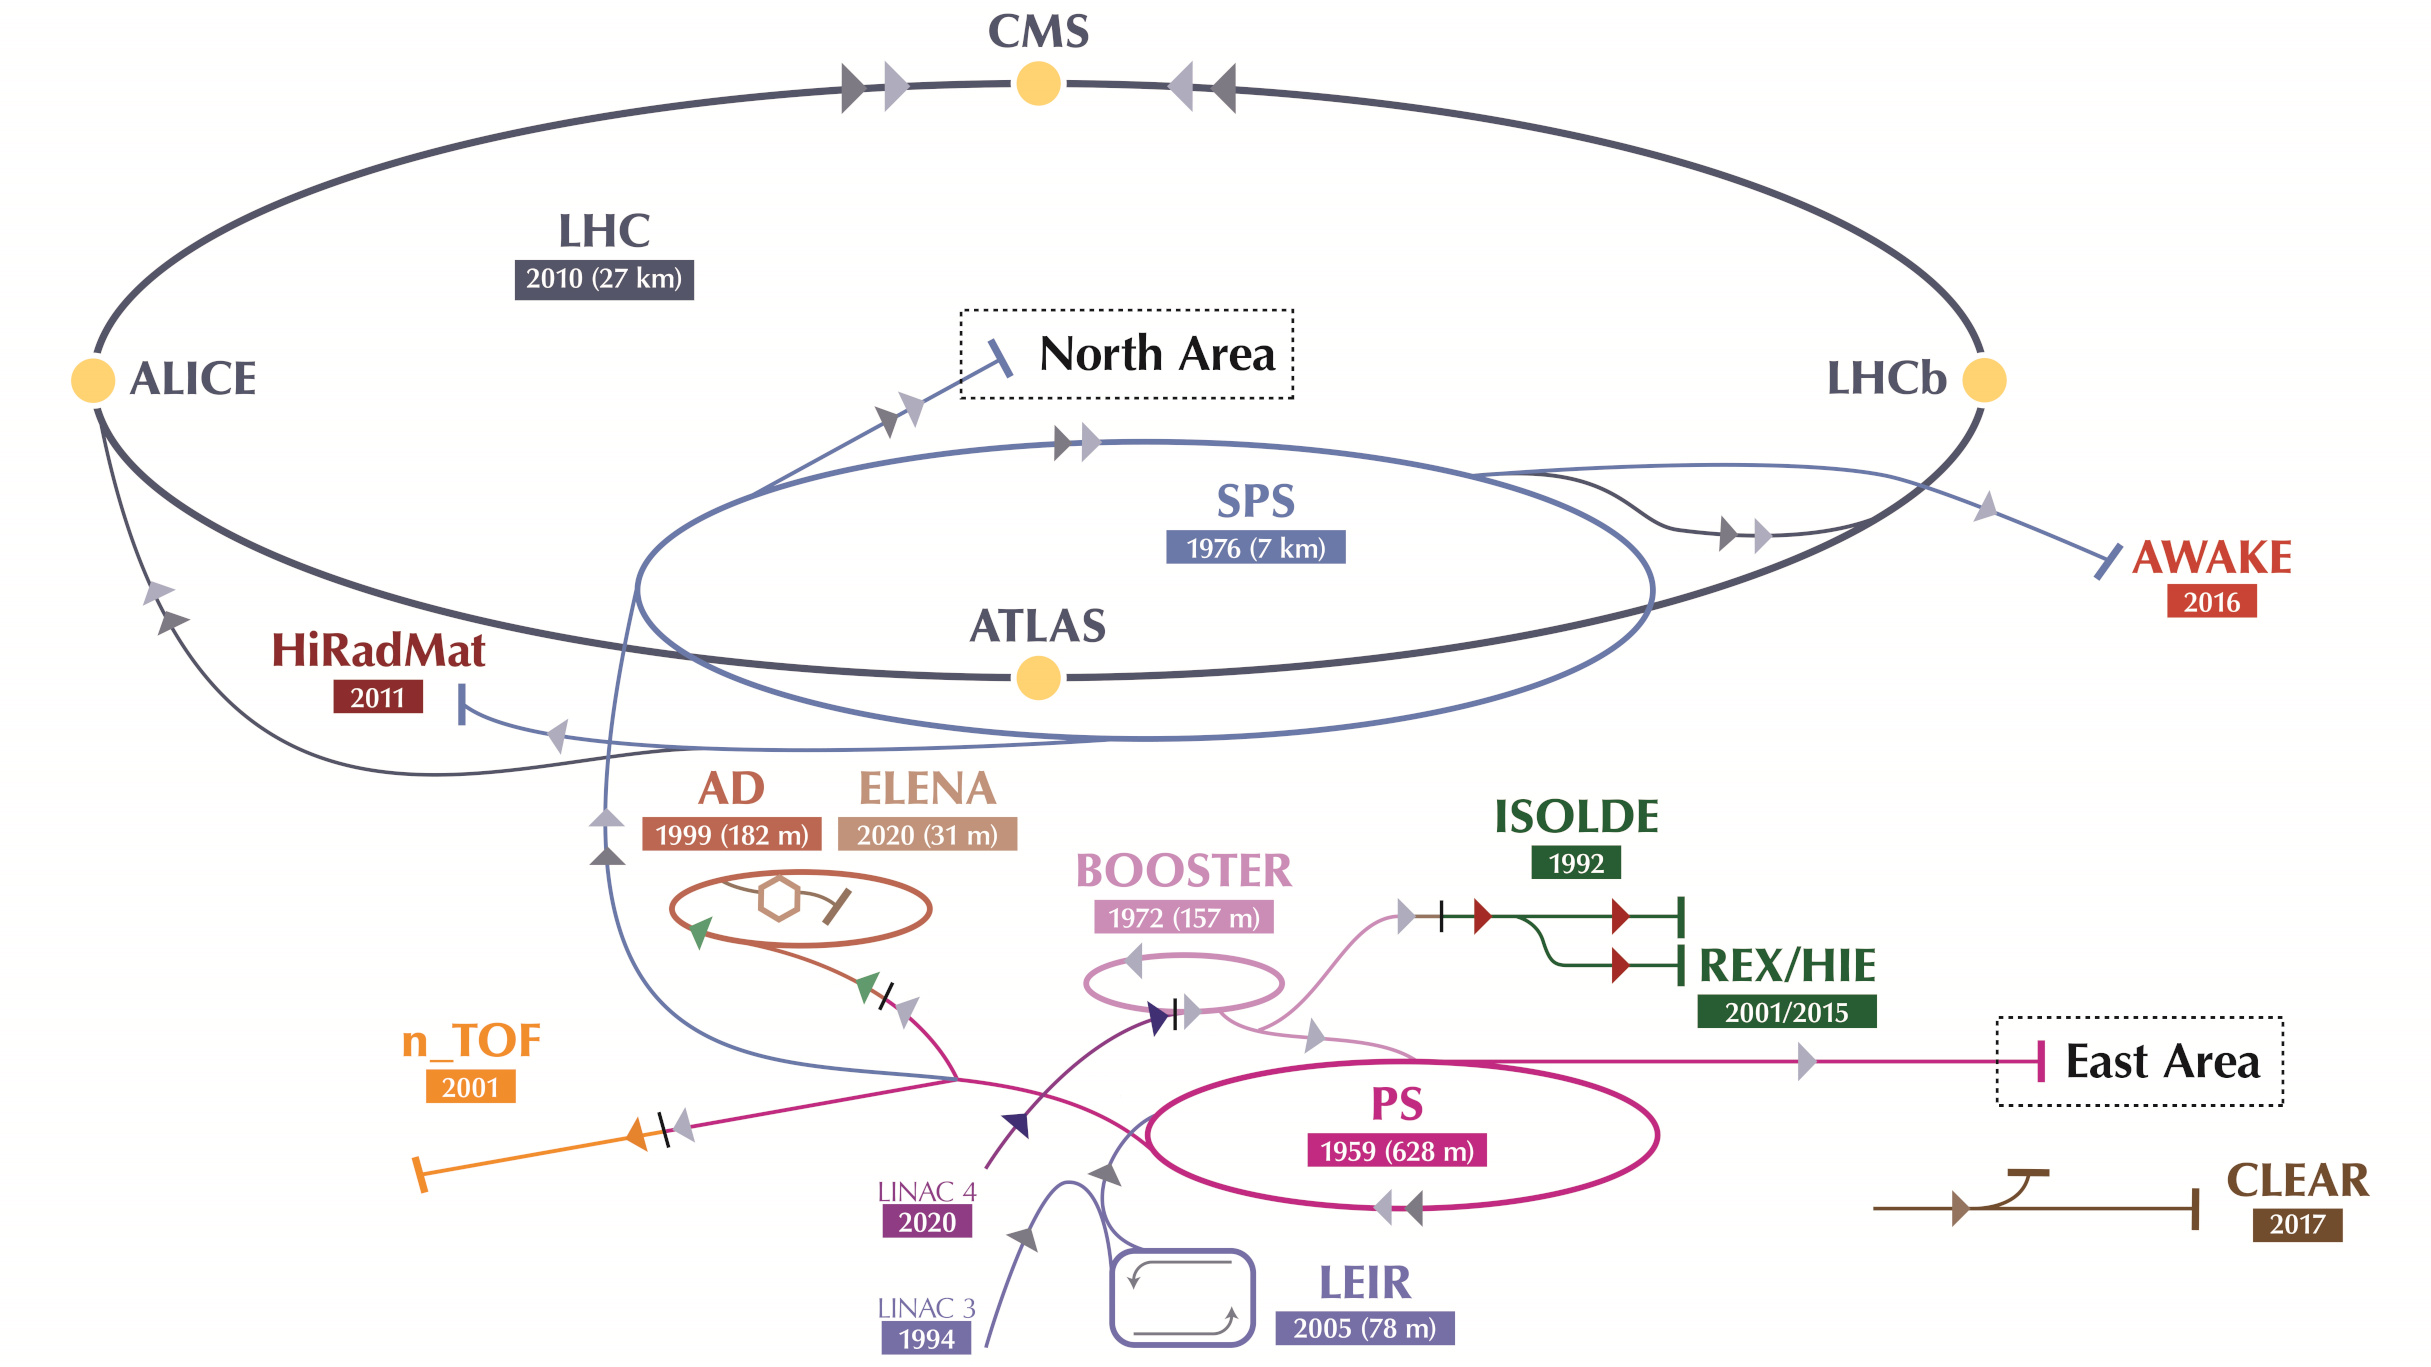
\includegraphics[scale=0.18]{Chapitre3/Images/cern-complex.jpg} 
\caption{Complexe d'accélérateurs du CERN \cite{CERNacc}.}
\label{complex}
\end{figure}

Le LHC est constitué d'une succession de 9593 électroaimants supraconducteurs parmis lesquels se trouvent 1232 aimants dipolaires de courbure fournissant chacun un champ magnétique de $8,3$ T. Chaque élément dipolaire mesure $15$ m et permet une courbure du faisceau de $0,6$ mm/m. Tout au long du parcours, 392 aimants quadripolaires assurent également la focalisation des faisceaux. Le régime supraconducteur des aimants, nécessitant une température de fonctionnement de $1,9$ K ($-271,3~^\circ$C) et un courant nominal de $12~000$ A, est maintenu grâce à un système de refroidissement cryogénique à l'hélium. Chaque faisceau circule dans un tube (\textit{beampipe}) distinct où un ultra vide correspondant à une pression de l'ordre de $10^{-13}$ atm est réalisé. Une fois l'énergie nominale atteinte, les faisceaux entrent en collision en quatre points correspondants aux emplacements des quatre grandes expériences du LHC. Lors de la première phase d'exploitation (Run 1) entre 2009 et 2012, l'énergie de collision dans le centre de masse était de $7$ TeV puis $8$ TeV avec un espacement des paquets de $50$ ns. Lors du Run 2 entre 2015 et 2018, l'énergie de collision a été augmentée à une valeur nominale de $13$ TeV et l'espacement réduit à $25$ ns. Enfin depuis le Run 3, l'énergie maximale de $6,8$ TeV par faisceau est atteinte, soit une énergie de collision de $13,6$ TeV. Le croisement de paquets de protons entraîne également l'apparition d'un phénomène d'empilement (PU, \textit{pile-up} désignant toutes les interactions secondaires prenant place conjointement à l'interaction principale (Fig. \ref{PU}). L'augmentation de la luminosité entraîne naturellement l'augmentation de l'empilement dont la valeur moyenne en juillet 2023 (Run 3) est de 49. \\

\begin{figure}
\centering
    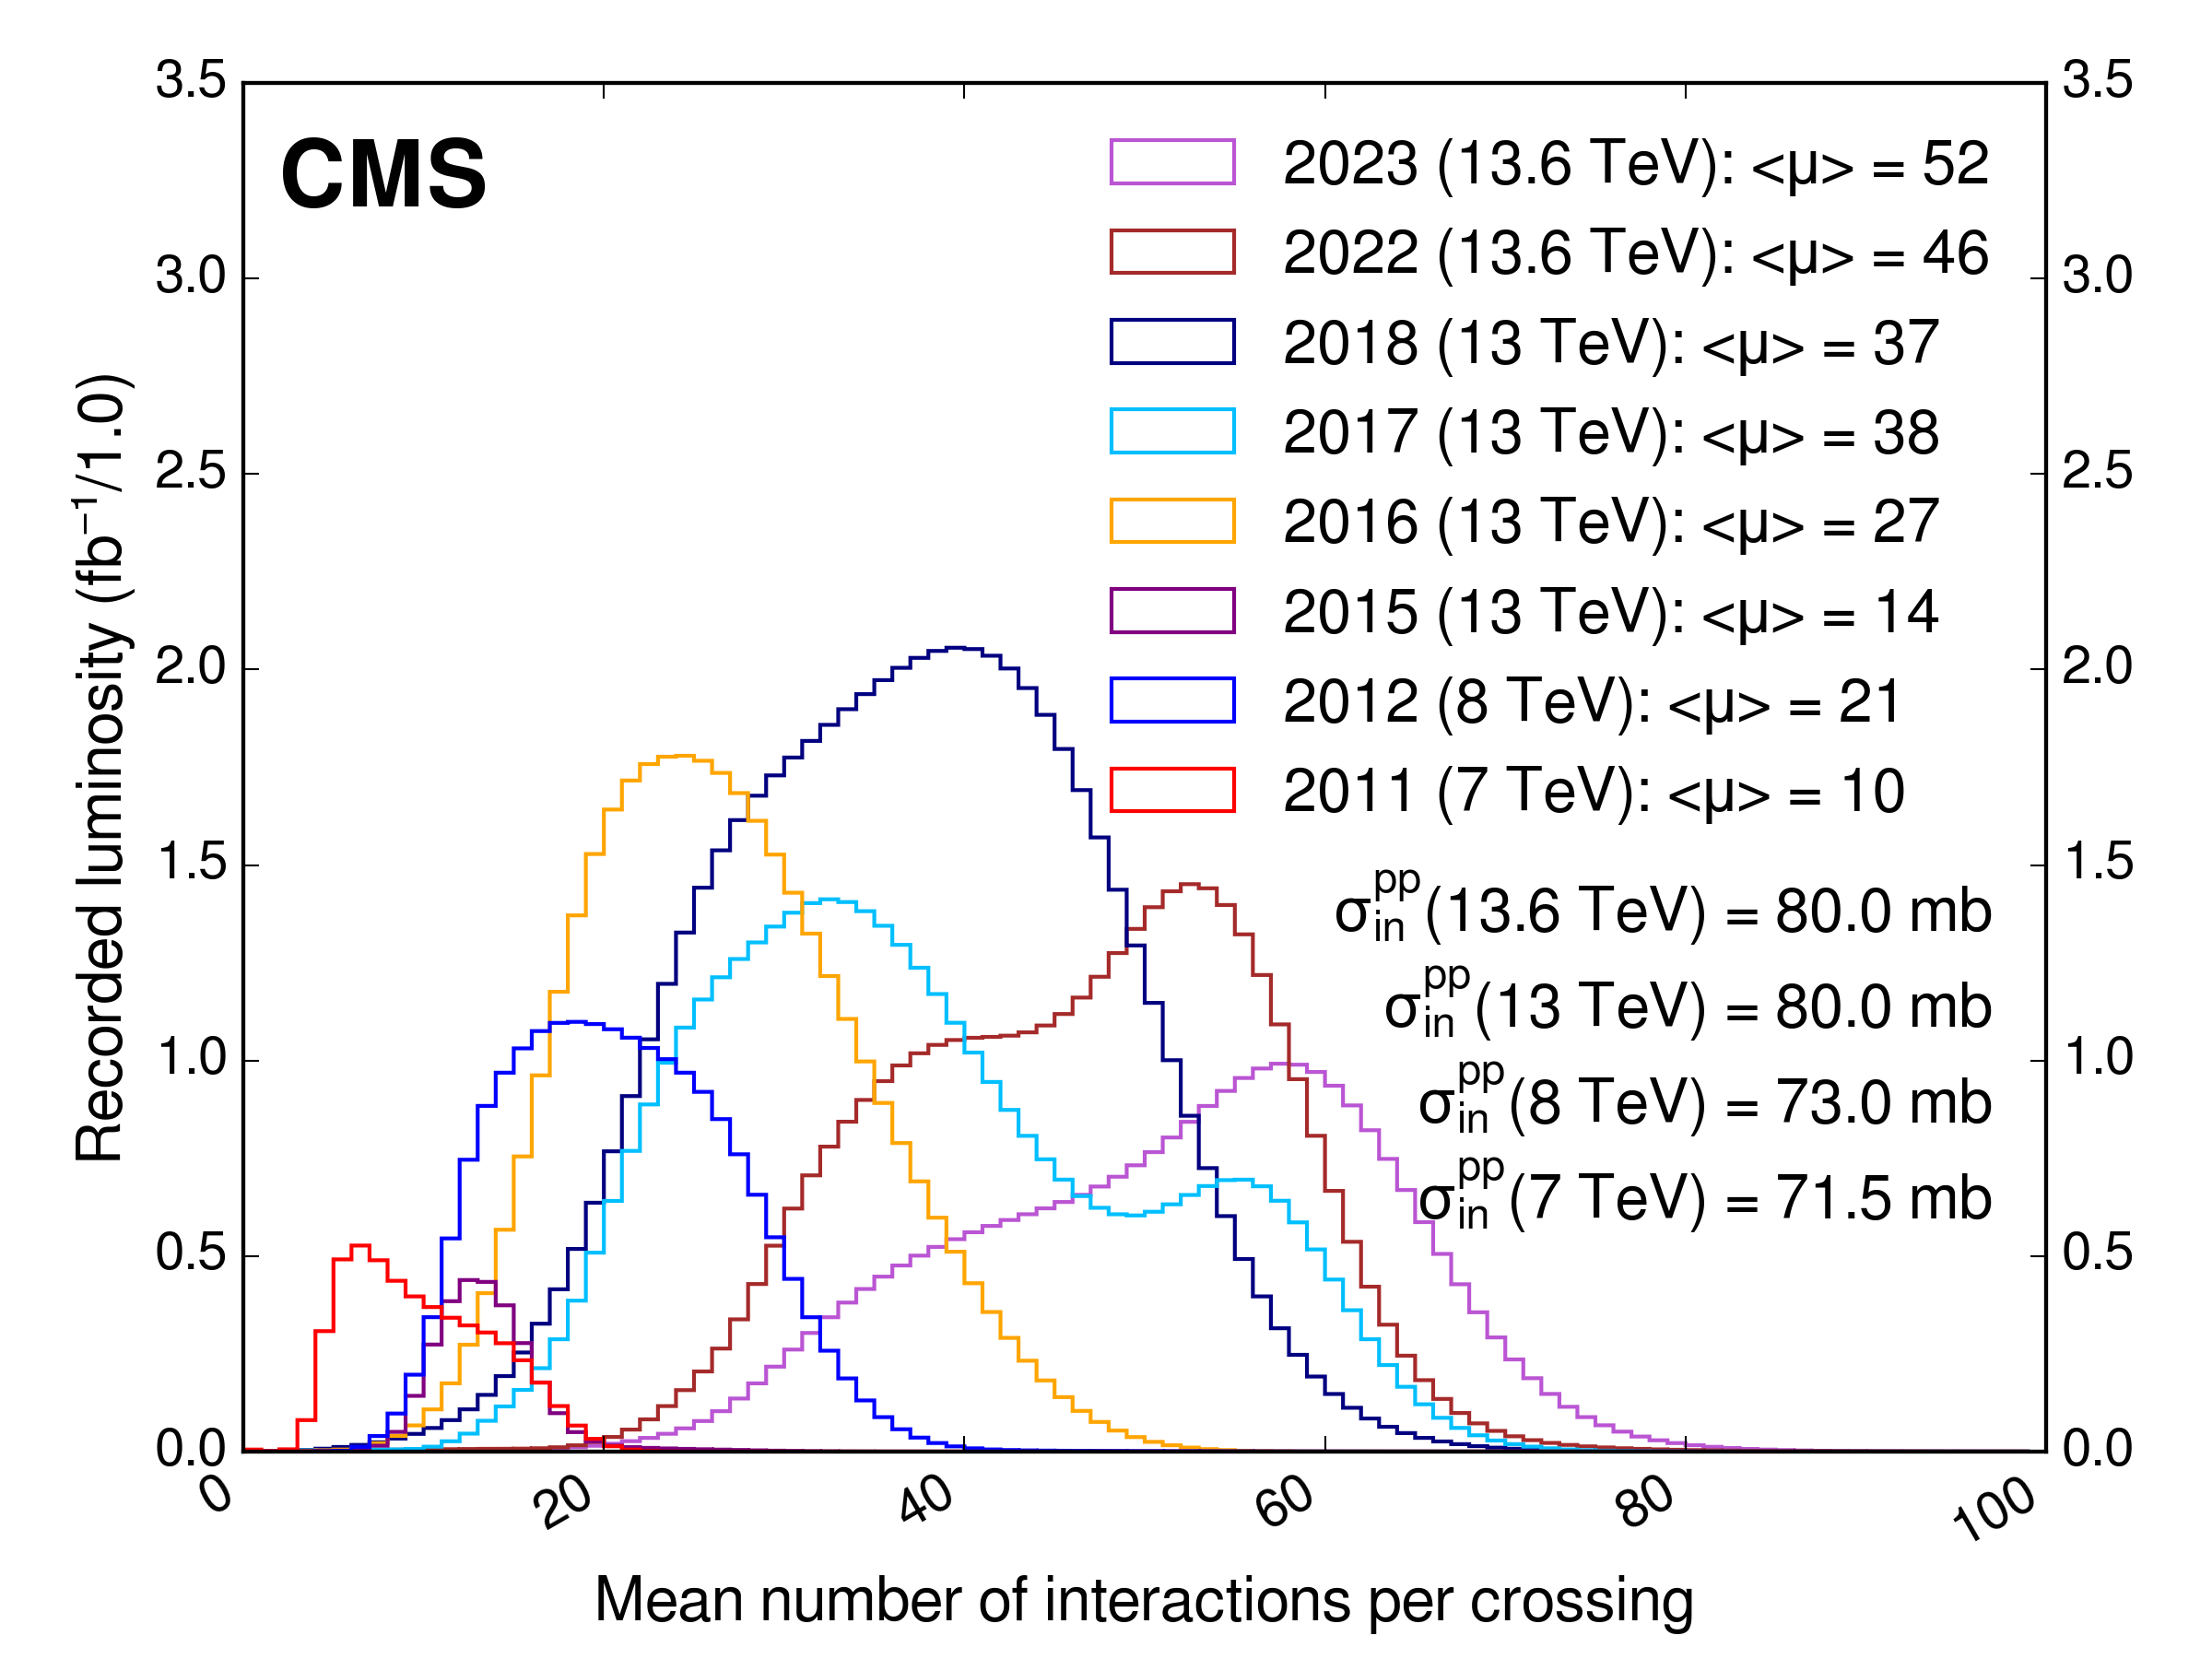
\includegraphics[scale=0.5]{Chapitre3/Images/pileup_allYears.png} 
\caption{Valeur moyenne de l'empilement par croisement de paquets de protons pour toutes les années d'exploitation du LHC \cite{LumiTwiki}.}
\label{PU}
\end{figure}

\section{Détecteur CMS, \textit{\uppercase{C}ompact \uppercase{M}uon \uppercase{S}olenoid}}

Le détecteur CMS, acronyme de \textit{Compact Muon Solenoid}, est un détecteur généraliste de forme cylindrique d'un diamètre de $15$ m et d'une longueur de $22$ m pour un poids total de $14~500$ t. Il est constitué de plusieurs sous-détecteurs et d'un aimant supraconducteur, disposés en couches concentriques (Fig. \ref{cms}), au centre desquelles le LHC délivre ses collisions. \\

\begin{figure}
\centering
    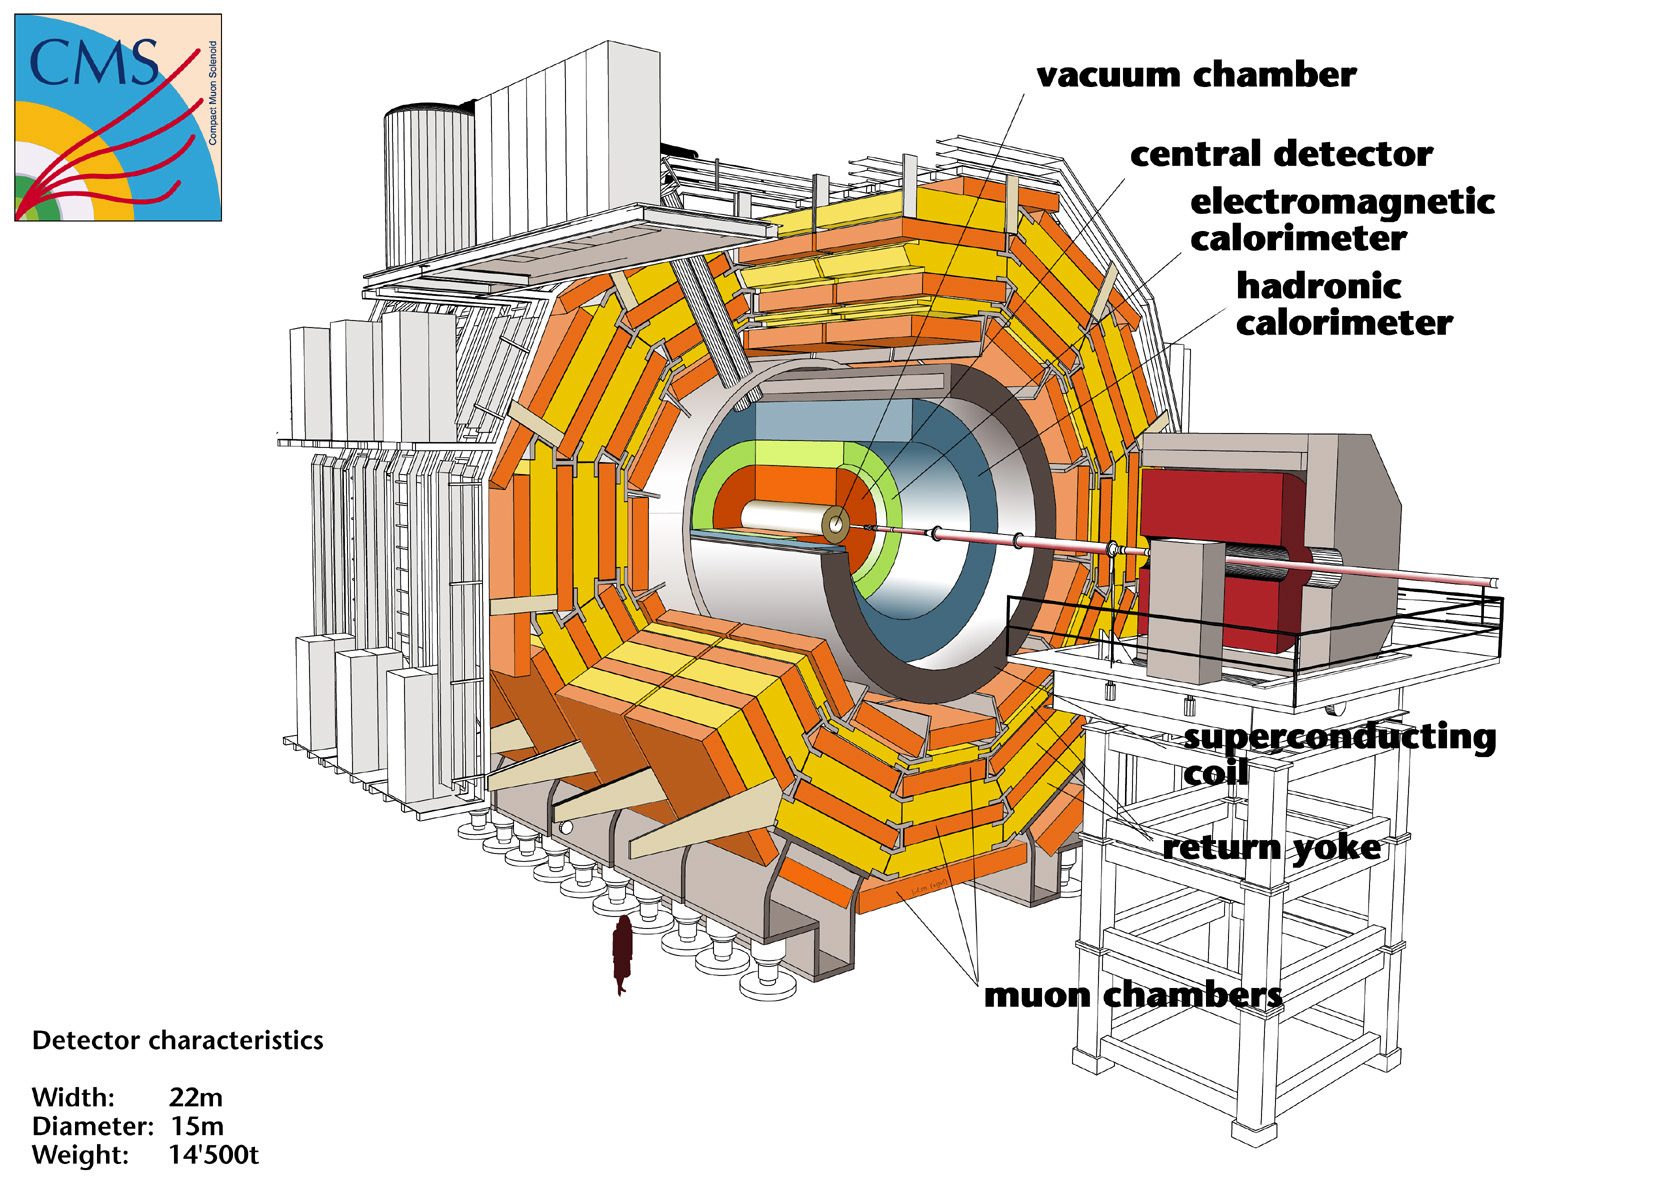
\includegraphics[scale=0.5]{Chapitre3/Images/CMS.jpg} 
\caption{Vue interne du détecteur CMS et de ses différents sous-détecteurs \cite{CMSscheme}.}
\label{cms}
\end{figure}

L'objectif d'un détecteur généraliste tel que CMS est de reconstruire et d'identifier une grande variété de particules issues des collisions produites en son centre. Les particules chargées sont identifiées à l'aide d'un champ magnétique de $3,8$ T fourni par un aimant solénoïde supraconducteur qui courbe leur trajectoire et par un système de trajectographie en silicium placé au centre du détecteur permettant de mesurer leur trajectoire et leur impulsion. L'énergie des particules neutres et chargées est mesurée grâce à un système de calorimétrie constitué d'un calorimètre électromagnétique (ECAL) et hadronique (HCAL). Enfin, CMS dispose d'un large système de trajectographie sur ses couches les plus externes dédié à l'identification et à la reconstruction des muons. 

\subsection{Système de coordonnées}

L'origine du système de coordonnnées de CMS (Fig. \ref{coordinates}) est défini au point d'interaction des faisceaux. L'axe $x$ pointe vers le centre de l'anneau du LHC, l'axe $y$ vers la surface terrestre et l'axe $z$ est orienté selon la direction du faisceau circulant en sens anti-horaire. Pour un vecteur d'impulsion $\vec{p}$ arbitraire, l'angle azimuthal $\phi$ désigne l'angle défini sur l'intervalle $[0;2\pi]$ entre la projection de $\vec{p}$ dans le plan $x$-$y$ et l'axe $x$. L'angle polaire $\theta$ désigne l'angle défini sur l'intervalle $[-\pi;\pi]$ entre $\vec{p}$ et l'axe $z$. Il est toutefois plus courant d'employer la pseudo-rapidité $\eta$ :

$$\eta = -\ln\bigl(\tan\frac{\theta}{2}\bigr).$$

Cette coordonnée est définie sur l'intervalle $]-\infty;+\infty[$, où chaque borne correspond à la direction selon l'axe $\pm z$, $\eta=0$ correspond à la direction selon l'axe $y$, et la différence $\Delta \eta$ entre deux particules est invariante de Lorentz. La pseudo-rapidité rentre également dans la définition de la séparation spatiale $\Delta R$ entre deux particules ou objets dans le plan $\eta$-$\phi$ définie comme :

$$\Delta R = \sqrt{\Delta\phi^2+\Delta\eta^2}.$$

La nature composite du proton ne permet pas de connaître l'impulsion selon l'axe $z$ des partons mis en jeu lors des collisions. En revanche cette impulsion est négligeable dans le plan transverse, et il convient ainsi de définir l'impulsion transverse : 

$$p_T=\sqrt{p_x^2+p_y^2},$$

dont la somme vectorielle $\Sigma\vec{p}_T^i$ sur chacune des particules $i$ de l'état final pour une collision donnée doit être nulle par conservation. Certaines particules comme le neutrino étant indétectables au sein du détecteur, on définit également l'impulsion transverse manquante :

$$\vec{p}^{miss}_T=-\Sigma\vec{p}_T^i,$$

correspondant à l'impulsion transverse totale des particules non observées. Aux régimes de haute énergie où la masse d'une particule est négligeable devant son impulsion, l'énergie transverse manquante $E^{miss}_T$, plus couramment désignée sous l'acronyme MET (\textit{Missing $E_T$}), s'exprime selon la relation :

$$E^{miss}_T=|\vec{p}_T^{miss}|.$$

\colorlet{veccol}{green!50!black}
\colorlet{myred}{red!70!black}
\colorlet{myblue}{blue!70!black}
\colorlet{mydarkred}{red!40!black}
\colorlet{mydarkblue}{blue!30!black}
\colorlet{CMScol}{red!80!black}
\colorlet{ATLAScol}{blue!80!black}
\tikzset{>=latex} % for LaTeX arrow head
\tikzstyle{axis}=[->,thick,line cap=round]
\tikzstyle{detector}=[thick,draw=mydarkred,rotate around z=\ang]
\tikzstyle{beam pipe}=[draw=blue!20!black!50,fill=blue!20!black!10,rotate around z=\ang]
\tikzstyle{detector surface}=[red!60!black!60,opacity=0.06,rotate around z=\ang]
\usetikzlibrary{angles,quotes} % for pic (angle labels)
\usetikzlibrary{bending} % for arrow head angle
%\newcommand*{\vv}[1]{\vec{\mkern0mu#1}} % aligned vector arrow

% CMS detector - left perspective
\tdplotsetmaincoords{75}{50} % to reset previous setting
\begin{figure}
\begin{tikzpicture}[scale=2.8,tdplot_main_coords,rotate around x=90]
  
  % VARIABLES
  \def\rvec{\L/2/cos(\thetavec)}
  \def\thetavec{18}
  \def\phivec{60}
  \def\L{3.3}    % detector length
  \def\R{0.75}   % detector cylinder radius
  \def\l{4.3}    % beam pipe length
  \def\r{0.04}   % beam pipe radius
  \def\rt{0.042} % beam pipe radius + line thickness
  \def\xmax{1}   % maximum x axis
  \def\ymax{1}   % maximum y axis
  \def\zmin{-\l/2-0.2} % minimum z axis
  \def\zmax{\l/2+0.3}  % maximum z axis
  \def\w{0.3}
  \coordinate (O) at (0,0,0);
  \coordinate (Z) at (0,0,\L/2);
  \tdplotsetcoord{O'}{0.022}{\thetavec}{\phivec} % slightly shifted origin
  \tdplotsetcoord{O''}{0.018}{90}{\phivec} % slightly shifted origin
  \tdplotsetcoord{P}{\rvec}{\thetavec}{\phivec}
  
  % CYLINDER behind
  \def\ang{19} % rotate lines to simulate cylinder
  \fill[top color=red!50!black!4,bottom color=red!60!black!2,rotate around z=\ang]
    (0,\R,\L/2) --++ (0,0,-\L) arc(90:270:\R) --++ (0,0,\L) arc(270:90:\R) -- cycle;
  \fill[detector surface] % transverse plane at z=L/2
    (0,0,\L/2) --++ (0,\R,0) arc(90:270:\R) -- cycle;
  \fill[detector surface] % transverse plane at z=-L/2
    (0,0,-\L/2) --++ (0,\R,0) arc(90:270:\R) -- cycle;
  \tdplotdrawarc[detector]{(0,0,\L/2)}{\R}{0}{360}{}{}
  \tdplotdrawarc[detector,thin]{(0,0,-\L/2)}{\R}{0}{360}{}{}
  %\draw[detector,canvas is yx plane at z=-\L/2] (0,0,0) circle(\R);
  \draw[detector,thin] % transverse plane at z=0
    (90-\ang:\R) arc (90-\ang:270:\R);
  \draw[detector] (0,0,-\L/2)++(90:\R) --++ (0,0,\L); % top horizontal
  \draw[detector] (0,0,-\L/2)++(-90:\R) --++ (0,0,\L); % bottom horizontal
  
  % BEAM PIPE
  \tdplotdrawarc[beam pipe]{(0,0,\l/2)}{\r}{0}{360}{}{}
  %\tdplotdrawarc[beam pipe]{(0,0,-\l/2)}{\r}{\ang-90}{90}{}{}
  %\draw[beam pipe] % cylindric beam pipe
  %  (0,\r,-\l/2) --++ (0,0,\l) arc(90:-90:\r)
  %  --++ (0,0,-\l) arc(-90:90:\r);
  \draw[beam pipe] % beam pipe, thinner in middle
    (0,\r,-\l/2) -- (0,\r,-0.2*\l) -- (90:0.5*\r)
    -- (0,\r,0.2*\l) -- (0,\r,0.5*\l) arc(90:-90:\r)
    -- (0,-\r,0.2*\l) -- (-90:0.5*\r) --
    (0,-\r,-0.2*\l) -- (0,-\r,-\l/2) arc(-90:90:\r);
  \draw[beam pipe] (0,0,\l/2) circle(\r);
  
  % AXES
  %\draw[thick,->] (0,0,0) -- (0,0,1) node[below right]{$z$}; % short
  \draw[axis,-] (0,0,\zmin) -- (0,0,0); % long
  \fill[CMScol] (O) circle(0.5pt) node[right=1,below=1] {};
  \draw[axis] (0,0,0.020) -- (0,0,\zmax) node[right=3,below=1]{$z$}; % long
  \draw[axis] (0,0.019,0) -- (0,\ymax,0) node[below left]{$y$};
  \draw[dashed,myred] (Px)  -- (Pxy);
  \draw[axis] (0.022,0,0) -- (\xmax,0,0) node[below=1,right=-2]{$x$};
  
  % LABELS
  \node[mydarkred,above] at (0,\ymax,0) {$\eta=0$};
  \node[mydarkred,above=3] at (0,\R,0.3*\L) {$\eta>0$};
  \node[mydarkred,above=3] at (0,\R,-0.2*\L) {$\eta<0$};
  \node[mydarkred,below=1,left] at (0,0,\zmax) {$\eta=\infty$};
  \node[mydarkred,above=1,right] at (0,0,\zmin) {$\eta=-\infty$};
  
  % VECTORS
  %\fill[radius=0.4,red] (P) circle;
  \draw[dashed,myred] (P)  -- (Pxy);
  \draw[dashed,myred] (Py) -- (Pxy);
  \draw[dashed,myred] (P) -- (Pz);
  \draw[->,red,line cap=round] (O') -- (P) node[anchor=-30] {$\vv{p}$};
  \draw[->,red,line cap=round] (O') -- (Pxy) node[anchor=-70] {$\vv{p}_{T}$};
  
  % CYLINDER front
  \draw[beam pipe,fill=none] (0,\r,-\l/2) arc(90:-90:\r);
  \fill[detector surface] % transverse plane at z=L/2
    (0,\rt,\L/2) --++ (0,\R-\rt,0) arc(90:-90:\R) --++ (0,\R-\rt,0) arc(-90:90:\rt);
  \fill[detector surface] % transverse plane at z=-L/2
    (0,\rt,-\L/2) --++ (0,\R-\rt,0) arc(90:-90:\R) --++ (0,\R-\rt,0) arc(-90:90:\rt);
  \tdplotdrawarc[detector]{(0,0,\L/2)}{\R}{-90}{90}{}{} % transverse plane at z=L/2
  \tdplotdrawarc[detector]{(0,0,-\L/2)}{\R}{-90}{90}{}{} % transverse plane at z=-L/2
  \draw[beam pipe,fill=none] (0,\r,\l/2) arc(90:-90:\r);
  \draw[detector,very thin] % transverse plane at z=0
    (90-\ang:\R) arc (90-\ang:-90:\R);
  
  % ANGLES
  \tdplotdrawarc[thick,red!57!black!3] % contour
    {(O)}{0.2}{4}{0.7*\phivec}{}{}
  \tdplotdrawarc[draw=none,opacity=0.8]{(O)}{0.2}{0}{\phivec} % transparant contour
    {above=2,right=-1,anchor=mid west}{\contour{red!55!black!3}{$\phi$}}
  \tdplotdrawarc[->]{(O)}{0.2}{0}{\phivec}
    {above=2,right=-1,anchor=mid west}{$\phi$}
  \tdplotdrawarc[->,rotate around z=\phivec-90,rotate around y=-90]
    {(O)}{0.88}{0}{\thetavec}{anchor=mid east}{$\theta$}
  \tdplotdrawarc[thick,red!58!black!4,rotate around z=\phivec-90,rotate around y=-90] % contour
    {(O)}{0.3}{88}{0.5*(90+\thetavec)}{}{}
  \tdplotdrawarc[-{>[flex'=1]},rotate around z=\phivec-90,rotate around y=-90,line cap=round]
    {(O)}{0.3}{90}{\thetavec}{above=4,right=2,anchor=mid east}{$\eta$}
  \draw[mydarkred] (0,0,\L/2) --++ (\R,0,0);
  \tdplotdrawarc[thick,red!60!black!6] % contour
    {(Z)}{0.2}{4}{0.7*\phivec}{}{}
  \tdplotdrawarc[draw=none,opacity=0.8]{(Z)}{0.2}{0}{\phivec} % transparant contour
    {above=2,right=-1,anchor=mid west}{\contour{red!60!black!6}{$\phi$}}
  \tdplotdrawarc[->]{(Z)}{0.2}{0}{\phivec}
    {above=2,right=-1,anchor=mid west}{$\phi$}
  
  % COMPASS - CMS-ATLAS axis has a ~12° declination
  \draw[->,thick,orange!30!black] (1.4*\w,-\R,-0.1*\L) --++ (2*\w,0,0)
    node[below=1,right,scale=0.8,align=center] {center of\\[-1pt]the LHC};

\end{tikzpicture}
\caption{Système de coordonnées du détecteur CMS \cite{izaak}.}
\label{coordinates}
\end{figure}


\subsection{Aimant supraconducteur}

L'aimant supraconducteur de CMS est un aimant solénoïde cylindrique d'un rayon de $6$ m et d'une longueur de $12,5$ m qui englobe au son centre le trajectographe en silicium et les calorimètres \cite{magnet1,magnet2}. Il est capable de délivrer un champ magnétique nominal de $3,8$ T et permet de courber la trajectoire des particules chargées afin d'en mesurer l'impulsion et la charge électrique. L'aimant et son champ magnétique sont eux mêmes confinés dans une culasse en fer permettant de créer un champ magnétique externe de $1,8$ T dans lequel se trouvent les chambres à muons. Le régime supraconducteur est maintenu grâce à un système de refroidissement à l'hélium liquide et une cuve à vide dans laquelle règne une température de $4,1$ K.

\subsection{Trajectographe en silicium}

La méthode de détection et de reconstruction de la trace des particules chargées dans le trajectographe de CMS, dont le détail est donné dans la section \ref{PF}, repose sur les propriétés de semi-conducteur du silicium. Par définition, un semi-conducteur est un matériau isolant dont l'écart modéré d'énergie entre sa bande de valence et sa bande de conduction permet le passage de courant sous certaines conditions. En particulier, l'énergie déposée par le passage d'une particule ionisante au sein d'un semi-conducteur peut suffire à la formation d'une paire électron-trou pouvant générer un courant par application d'un champ électrique externe. Dans le cas du silicium l'énergie minimale requise pour la formation d'une paire électron-trou est de $3,6$ eV, ainsi le passage d'une particule au minimum d'ionisation (MIP) entraîne la formation de $80$ paires/$\mu$m. Pour un détecteur d'une épaisseur de $300$ $\mu$m, ce même passage entraînera la formation d'environ $2\times10^4$ électrons, indiscernables parmi une densité de porteurs intrinsèques du silicium d'environ $10^{10}$ cm$^{-3}$. La formation d'une zone de déplétion dépourvue de charges libres au sein du matériau est ainsi cruciale pour permettre la détection de particules chargées. \\

La conductivité du silicium peut être améliorée par une technique de dopage consistant à insérer au sein de sa maille cristalline des atomes étrangers donneurs (type III) ou accepteurs (type V) d'électrons. Lorsqu'un matériau de type III est employé, le silicium est enrichi en électrons et possède un dopage de type $n$. A l'inverse, un matériau de type V entraîne un déficit d'électrons au sein du silicium et constitue un dopage de type $p$. Les détecteurs en silicium sont généralement conçus à partir d'un volume de type $n$ sur lequel une couche de type $p$ sur laquelle les charges sont collectées est déposée. La zone de contact formée constitue une jonction dite $p$-$n$, au niveau de laquelle une zone de déplétion dépourvue de charges se crée par des effets de migration entre les deux couches. Par ailleurs, au sein d'un détecteur, la jonction $p$-$n$ est généralement opérée en régime de polarisation inverse en appliquant un champ électrique généré par une tension externe dont la cathode est reliée au volume $n$ et l'anode à la couche $p$. Cette méthode permet non seulement d'élargir la zone de déplétion qui constitue la zone active du détecteur proportionnellement à la tension appliquée, mais également de prévenir la fuite de charges à l'origine du bruit. Une couche de type $n^+$, plus fortement dopée, peut également être déposée sur la face opposée du volume de type $n$ afin d'augmenter davantage l'effet de déplétion. \\

Le trajectographe de CMS est un cylindre constitué de couches de détection concentriques successives dans sa partie centrale (tonneau), et d'un empilement de disques dans ses parties avants (bouchons) permettant de couvrir la région définie par $r<1,2$m et $|\eta|<2,5$ (Fig. \ref{tracker}). Le détecteur est entièrement équipé de modules en silicium, avec sa partie interne constituée de pixels, et sa partie externe constituée de modules à micro-pistes. \\

\begin{figure}
\centering
    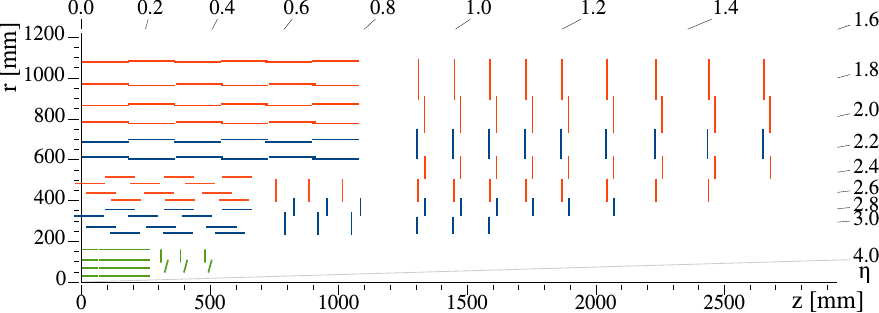
\includegraphics[scale=0.95]{Chapitre3/Images/Phase1_Tracker_1Quarter.png} 
\caption{Quart de coupe dans le plan $r$-$z$ du trajectographe Phase-1 de CMS. Les pixels sont représentés en vert, les modules à pistes simple face en rouge et les modules à pistes double face en bleu \cite{TrackerPerformance}.}
\label{tracker}
\end{figure}

\subsubsection{\ding{95} Trajectographe à pixels}

Les détecteurs à pixels sont constitués d'un volume actif en silicium dopé sur lequel une couche de type inverse et segmentée en "pixels" est déposée. En ajoutant une piste de lecture à chaque segment, les pixels agissent comme des détecteurs individuels et offrent une excellente granularité. Dans le cas de CMS, le volume actif des modules est composé d'un volume de type $n$ surplombé d'une couche de type $n^+$  et d'une couche de type $p$ sur sa face opposée. Une fois opérée en polarisation inverse, cette configuration permet de collecter des électrons sur les pixels plutôt que des trous. Ces derniers possèdent en effet une mobilité plus faible que les électrons et sont ainsi davantage sujets aux effets de capture causés par les dommages liés à la forte exposition aux radiations. En 2017, la Phase-$0$ du trajectographe de CMS s'est achevée pour laisser place à la Phase-$1$ prévue pour être opérée jusqu'à la fin du Run 3. Durant cette phase de jouvence du détecteur, une couche supplémentaire de pixels a été ajoutée dans le tonneau (BPIX, \textit{barrel pixels}), portant à 4 le nombre total de couches concentriques situées respectivement à $r=30,68,109,160$ mm. Les bouchons (FPIX, \textit{forward pixels}) sont quant à eux constitués de trois disques couvrant la région située dans un rayon compris entre $45$ et $161$ mm. Au total, le trajectographe à pixels est constitué de $1856$ modules silicium pour un total de $100$ millions de pixels d'une taille de $100\times150$ $\mu$m$^2$. La résolution sur la reconstruction des \textit{hits} individuels des traces de particules chargées est de $10$ $\mu$m dans le BPIX et de $15$ $\mu$m dans le FPIX.

\subsubsection{\ding{95} Trajectographe à pistes}

Les modules à micro-pistes sont constitués d'un volume actif de type $n$ sur lequel sont implantées des bandes de type $p^+$. Le trajectographe à pistes est constitué d'une partie interne comprenant un tonneau (TIB, \textit{Tracker Inner Barrel}) constitué de quatre couches, et de deux bouchons (TID, \textit{Tracker Inner Disks}) constitués de trois disques sur les parties avants. Chaque module de la partie interne possède une épaisseur de $320$ $\mu$m et un espacement entre chaque piste de $80$ $\mu$m. La partie externe comporte quant à elle six couches dans son tonneau (TOB, \textit{Tracker Outer Barrel}) et neuf disques dans chacun de ses bouchons (TEC, \textit{Tracker EndCaps}). Les modules de la partie externe possèdent une épaisseur de $500$ $\mu$m et un espacement entre les pistes de $205$ $\mu$m. \\

\begin{figure}
    \begin{subfigure}[b]{0.5\linewidth}
    \centering
    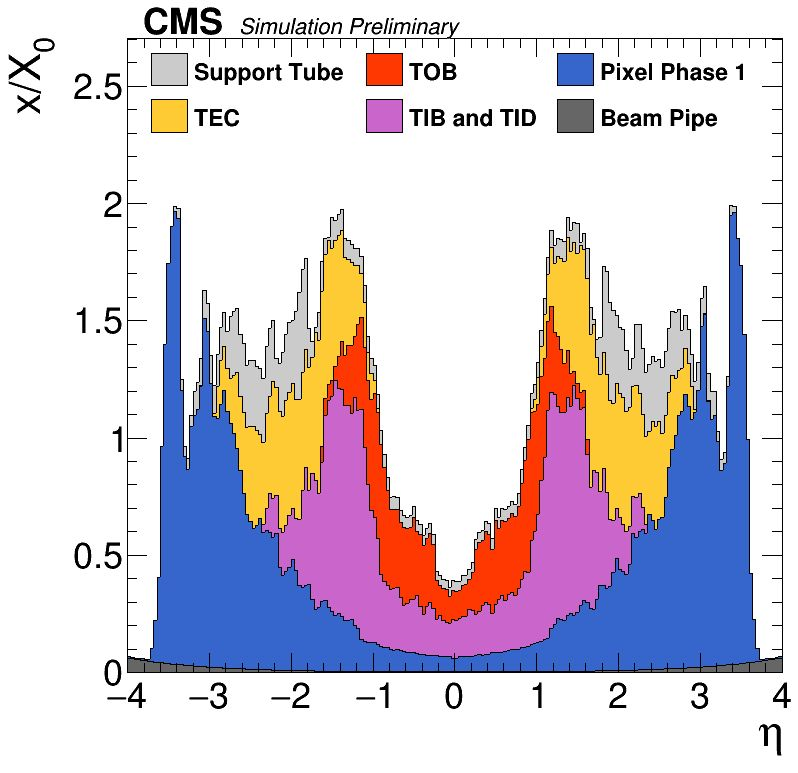
\includegraphics[width=\linewidth]{Chapitre3/Images/MaterialBudgetTrackerPhase1_FractionRadiationLength.png} 
    \caption*{} 
    \vspace{0.5ex}
  \end{subfigure}%% 
  \begin{subfigure}[b]{0.5\linewidth}
    \centering
    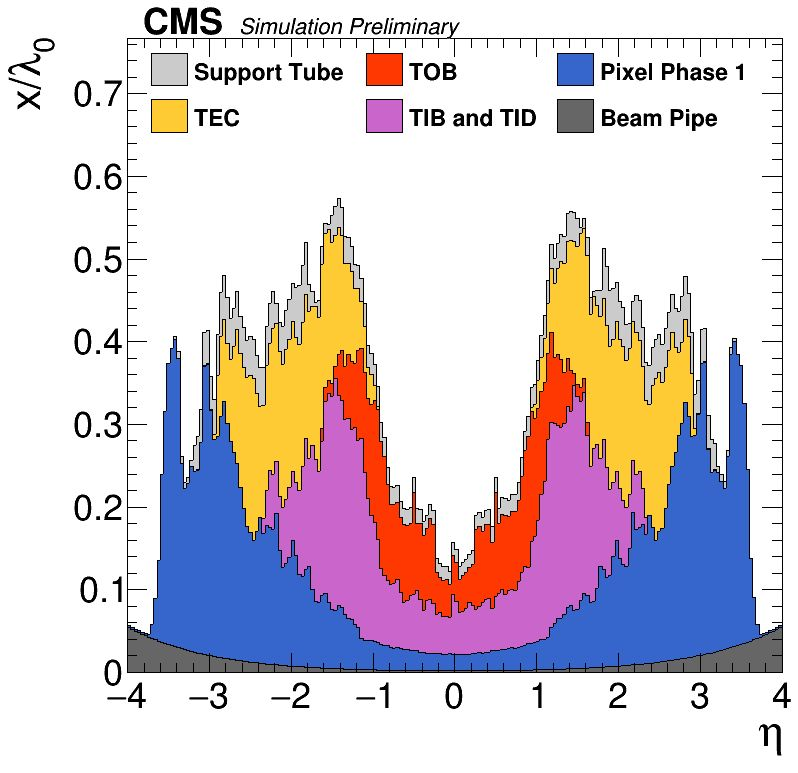
\includegraphics[width=\linewidth]{Chapitre3/Images/MaterialBudgetTrackerPhase1_HadronicInteractionLengthFraction.png} 
    \caption*{} 
    \vspace{0.5ex}
  \end{subfigure}
  \caption{Budget de matière du trajectoraphe de CMS en fonction de $\eta$ exprimé en unité de longueur de radiation (gauche) et de longueur d'interaction hadronique (droite) \cite{TrackerBudget}.}
  \label{materialbudget}
\end{figure}

L'intégralité du trajectographe est équipée d'un système de refroidissement permettant de limiter les dégats causés par les radiations ainsi que le bruit électronique. Plusieurs interactions entre rayonnement et matière sont également à l'origine de la modification de la trajectoire des particules et d'une perte d'énergie non mesurable au sein du trajectographe. Parmi ces effets, on compte notamment la conversion des photons en paire électron-positron, le rayonnement de freinage des électrons, les interactions nucléaires des hadrons et la diffusion mutliple sur les noyaux de silicium. Pour limiter ces effets, le budget de matière du détecteur (Fig. \ref{materialbudget}) doit être minimal. 

\subsection{Calorimétrie}

Le système de calorimétrie de CMS est composé de deux sous-détecteurs : un calorimètre électromagnétique (ECAL) et un calorimètre hadronique (HCAL) dont la première fonction commune est de stopper et de mesurer l'énergie des particules incidentes. Tandis que le premier est chargé de mesurer l'énergie des photons et des électrons, le second permet de mesurer l'énergie des particules hadroniques interagissant par interaction forte. Dans les deux cas, le principe de mesure repose sur la conversion d'une particule incidente en une cascade de particules de plus faibles énergies qui a leurs tours sont converties en photons par un matériau scintillant. Ces photons sont par la suite collectés par un photo-multiplicateur permettant de produire un signal électrique proportionnel à l'énergie déposée.  

\begin{figure}
\centering
    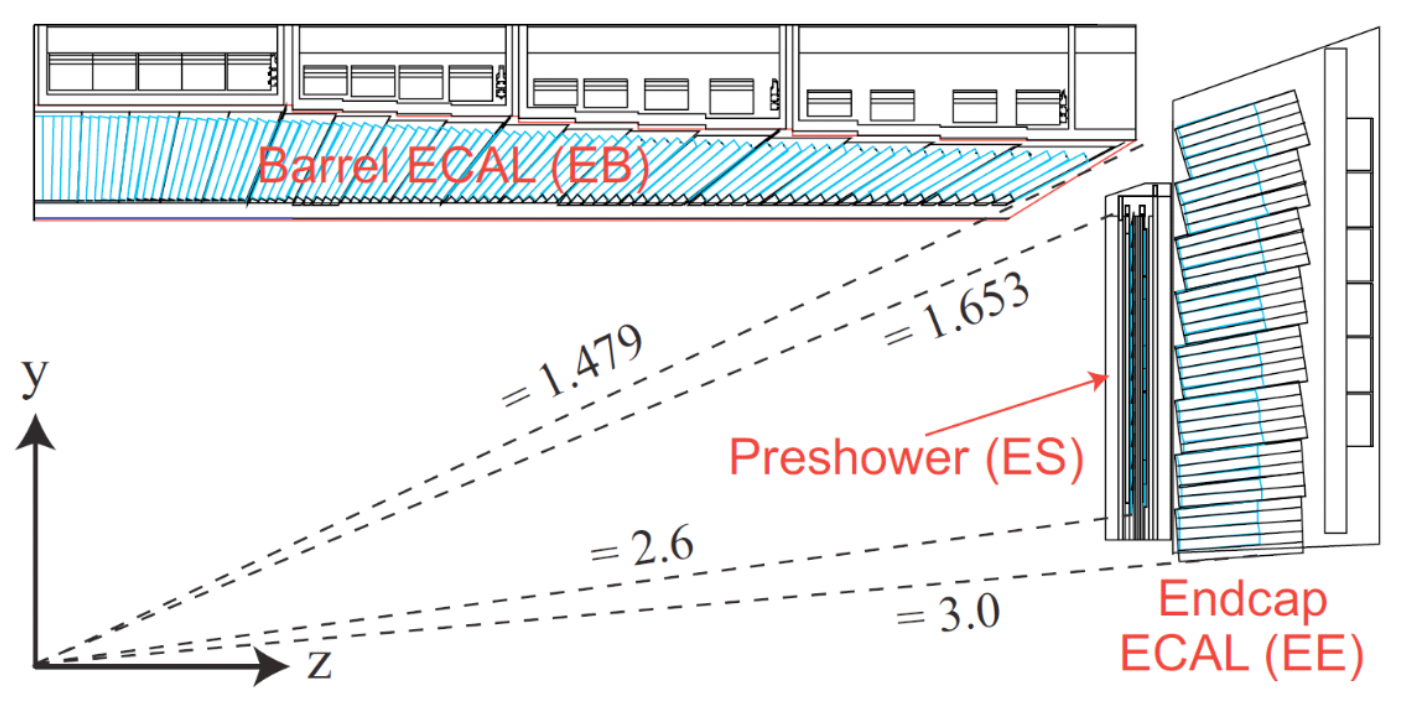
\includegraphics[scale=0.28]{Chapitre3/Images/ECAL.png} 
\caption{Quart de coupe dans le plan $r$-$z$ du calorimètre électromagnétique de CMS \cite{ECAL}.}
\label{ecal}
\end{figure}

\subsubsection{\ding{95} Calorimètre électromagnétique (ECAL)}

Le calorimètre électromagnétique de CMS est un calorimètre homogène dont les modules sont entièrement composés de cristaux de stolzite (\chemform{PbWO_4}) et dans lequel l'énergie des électrons et des photons est mesurée. Ce cristal possède l'avantage d'une bonne résistance aux radiations, d'une courte longueur de radiation $X_0=0,89$ cm correspondant à la distance après laquelle l'énergie d'un électron incident est réduite d'un facteur $1/e$, d'un faible rayon de Molière de $2,2$ cm défini comme le rayon d'un cylindre contenant $90\%$ de l'énergie d'une gerbe et d'un temps de réponse de seulement $15$ ns. L'ECAL constitue la couche de détection suivant le trajectographe et contient deux parties principales : un tonneau cylindrique (EB, \textit{ECAL Barrel)}) couvrant la région définie par $|\eta|<1,479$ et deux bouchons (EE, \textit{ECAL Endcaps}) couvrant la région définie par $1,479<|\eta|<3$ (Fig. \ref{ecal}). Le tonneau et les bouchons se composent d'un total de $75~848$ cristaux, dont $61~200$ d'une longueur de $25,8X_0$ dans le tonneau et $7~324$ d'une longueur de $24,7X_0$ dans les bouchons avec chacun une segmentation $\Delta\phi\times\Delta\eta=0,0175\times0,0175$. Ces dimensions permettent à chaque cristal de contenir l'intégralité d'une gerbe électromagnétique produite par une particule incidente et de fournir une estimation de sa direction. Les parties avants du calorimètre sont également équipées d'un système de \textit{preshowering} (ES) placés avant les bouchons dont la granularité élevée permet de différencier un photon seul de deux photons issus de la désintégration d'un pion neutre lorsque ce dernier est fortement boosté. La résolution en énergie $\sigma_E$ du ECAL a été mesurée dans les données à $7$ TeV \cite{ECALres} comme étant :

\begin{equation}
    \frac{\sigma_E}{E}=\frac{0.027}{\sqrt{E}}+\frac{0.12}{E}+0.005,
\end{equation}

avec $E$ l'énergie mesurée et où le premier terme est un terme stochastique issu des fluctuations statistiques de l'énergie des gerbes électromagnétiques, le second est relié au bruit et à l'empilement et le troisième est un terme tenant compte des imperfections du détecteur et des fuites d'énergie.

\begin{figure}
\centering
    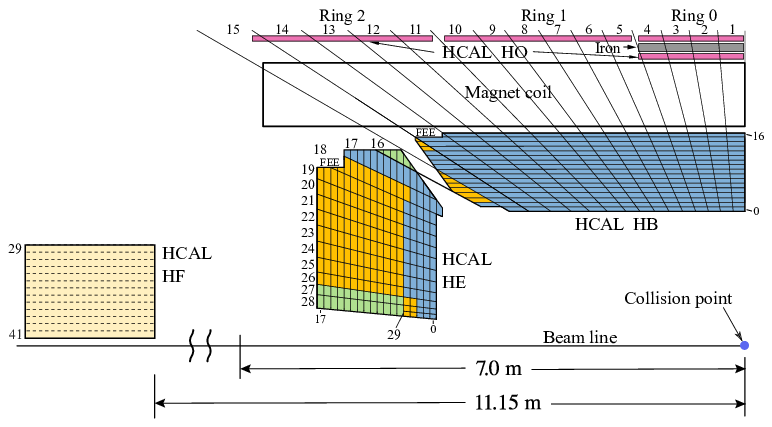
\includegraphics[scale=0.5]{Chapitre3/Images/HCAL.png} 
\caption{Quart de coupe dans le plan $r$-$z$ du calorimètre hadronique de CMS \cite{HCAL}.}
\label{hcal}
\end{figure}

\subsubsection{\ding{95} Calorimètre hadronique (HCAL)}

Le calorimètre hadronique de CMS est un calorimètre inhomogène constitué de couches successives de matériau absorbant dans lequel se forment les cascades et de matériau scintillant. La partie principale du HCAL se situe immédiatement après le ECAL et contient un tonneau (HB, \textit{HCAL Barrel}) couvrant la région $|\eta|<1,4$ et deux bouchons (HE, \textit{HCAL Endcaps}) couvrants la région $1,3<|\eta|<3$ (Fig. \ref{hcal}). Le tonneau et les parties avants contiennent chacune $2~304$ modules d'une résolution $\Delta\phi\times\Delta\eta=0,087\times0,087$ constitués de couches successives de laiton et de plastique scintillant. Une seconde partie du HCAL est également située à l'extérieur de l'aimant pour les particules les plus énergétiques avec une partie centrale (HO, \textit{Outter HCAL}) dans la région $|\eta|<1,3$ et de deux parties avants (HF, \textit{Forward HCAL}) dans la région $2,9<|\eta|<5,2$ (Fig. \ref{hcal}). Tandis que le HO utilise également un plastique scintillant comme matériau actif, le HF requiert une meilleure résistance aux radiations et utilise un matériau constitué de fibres de quartz. Pour ces deux parties externes la culasse en fer de l'aimant joue le rôle d'absorbeur. La résolution en énergie $\sigma_E$ en fonction de l'énergie mesurée $E$ des parties constituées de plastique scintillant est donnée par :

\begin{equation}
    \frac{\sigma_E}{E}=\frac{0,9}{\sqrt{E}}+0.045,
\end{equation}

tandis que celle du HF seul est donnée par :

\begin{equation}
    \frac{\sigma_E}{E}=\frac{1,72}{\sqrt{E}}+0.09.
\end{equation}

\subsection{Chambres à muons}

Les muons interagissent peu avec la matière et volent suffisamment longtemps pour s'échapper du détecteur. Les chambres à muons constituent ainsi les dernières couches de détection de CMS placées après l'aimant supraconducteur et sont soumises à un champ magnétique de $1,8$ T grâce à la culasse de retour en fer de ce dernier. Elles sont composées de détecteurs gazeux dont l'ionisation par les muons incidents permet la reconstruction de leur trace et de leur impulsion en combinant les informations du trajectographe en silicium central. 

\begin{figure}
\centering
    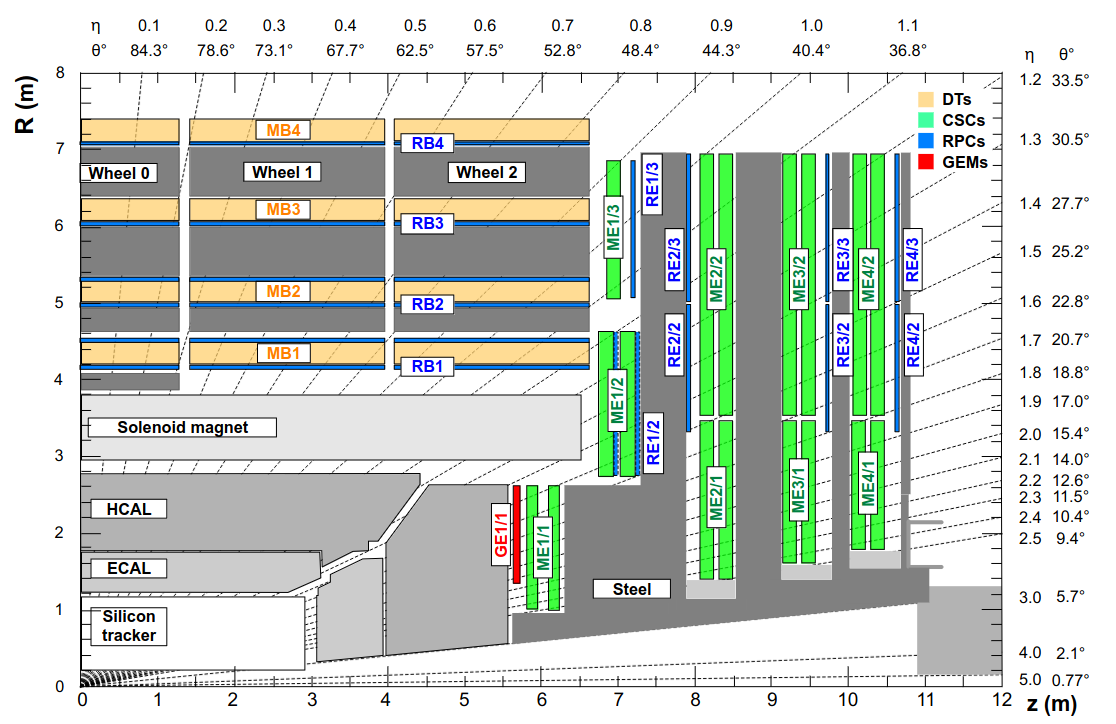
\includegraphics[scale=0.37]{Chapitre3/Images/MUONS.png} 
\caption{Quart de coupe dans le plan $r$-$z$ du système de chambres à muons de CMS \cite{MUONS}.}
\label{muons}
\end{figure}

\subsubsection{\ding{95} Tubes à dérive (DT)}

Les tubes à dérive couvrent la région centrale du détecteur lorsque $|\eta|<1,2$. Chaque élément consiste en un tube creux de section rectangulaire d'environ $1,3\times4,2$ cm$^2$ et rempli de gaz ($85\%$ \chemform{Ar}, $15\%$ \chemform{CO_2}) dans lequel un fil métallique est tendu. Lorsqu'une particule chargée traverse ce volume, elle ionise le gaz présent et l'application d'un champ électrique permet la dérive et la collecte des charges produites sur le fil central qui après amplification génèrent un signal électrique mesurable. La mesure du temps de dérive des électrons au sein du tube permet également de reconstruire une information $2D$ du passage de la particule. Dans CMS, plusieurs de ces tubes sont répartis en couches empilées et quatre couches forment une "super-couche" (\textit{superlayer}). Ces \textit{superlayers} contiennent chacune jusqu'à $90$ tubes et sont elles-mêmes placées par $3$ dans des chambres dont la dimension varie de $2\times2,5$ m$^2$ à $4\times2,5$ m$^2$. Une mesure $3D$ de la trace est obtenue en combinant les informations des différentes \textit{superlayers} au sein d'une chambre : la couche centrale mesure la coordonnée parallèle à l'axe du faisceau et les deux couches externes la coordonnée perpendiculaire avec une résolution spatiale de $100$ $\mu$m.

\subsubsection{\ding{95} Chambres à fils cathodiques (CSC)}

Les chambres à fils cathodiques se situent dans les parties avants de CMS et couvrent la région $0,9<|\eta|<2,4$. Ces dernières sont plus adaptées pour une forte exposition aux radiations et sont constituées, à l'image des chambres à fils, d'anodes filaires croisées à des pistes cathodiques dans un volume de gaz ($40\%$ \chemform{Ar}, $50\%$ \chemform{CO_2}, $10\%$ \chemform{CF_4}).

\subsubsection{\ding{95} Chambres à plaques résistives (RPC)}

Les RPC sont constituées de deux plaques de bakélite séparées par un volume fin de quelques millimètres d'épaisseur et rempli de gaz. Un champ électrique est appliqué entre les deux plaques de forte résistivité, et les charges produites par ionisation lors du passage d'une particule chargée sont collectées par des bandes métalliques externes. Ce système de détection possède une résolution spatiale moindre mais un temps de réponse particulièrement court inférieur à $25$ ns. Les RPC sont ainsi utilisées en complément des CSC et des DT dans le système de déclenchement du détecteur. \\

Un nouveau type de détecteur gazeux appelé \textit{gas electron mutiliplier} (GEM) est également venu récemment compléter le système de chambres à muons de CMS \cite{GEM1,GEM2}. Les GEMs ont pour but d'améliorer la détection des muons dans les parties avants du détecteur en couvrant la région $1,6<|\eta|<2,2$ en prévision de l'augmentation de l'empilement et de l'exposition aux radiations. Un total de $144$ modules a été installé avant le lancement du Run 3 dans le premier disque de chaque bouchons de CMS et les deux disques suivants seront à leur tour équipés lors du lancement de la phase à haute luminosité. 

\subsection{Système de déclenchement}

Depuis le début du Run 2, le LHC délivre des collisions avec un croisement de paquets de protons toutes les $25$ ns. Ces collisions produisent jusqu'à $40$ millions d'évènements par seconde dont la plupart ont peu d'intérêt physique. Le système de déclenchement de CMS \cite{triggersystem} permet de filtrer ces évènements en conservant ceux répondant aux critères jugés intéressants pour les interactions à étudier et ainsi de réduire la quantité de données à stocker. Ce système de déclenchement, aussi désigné par \textit{trigger}, contient un premier niveau L$1$ (\textit{Level 1 Trigger}) et un second niveau HLT (\textit{high level trigger}). \\

Le niveau L$1$ est un système de déclenchement purement électronique qui s'appuie sur les informations délivrées par les calorimètres et les chambres à muons sans reconstruction de traces. Les conditions selon lesquelles un évènement est conservé ou non peuvent inclure des limites cinématiques ou requérir la présence de certains objets et sont regroupées au nombre de 256 au sein d'un "menu" sous le nom de \textit{L1 seeds}. Pour chaque évènement, seulement 3,4 $\mu$s sont nécessaires à la prise de décision de l'électronique et le niveau L$1$ permet de réduire la fréquence des évènements de $40$ MHz à environ $100$ kHz. \\

Le niveau $HLT$ traite ensuite par un algorithme les évènements conservés par le niveau $L1$ en effectuant une reconstruction rapide de l'évènement et en associant les dépôts d'énergie des calorimètres à des traces grâce aux informations du trajectographe en silicium central. Les critères de sélection du niveau $HLT$ regroupés sous forme de \textit{chemins} permettent de réduire la fréquence des évènements à $1$ kHz et ces derniers sont stockés. \\